In diesem Kapitel wird auf die Ergebnisse der Evaluation eingegangen. Zudem wird auf die Benchmarks der CPU und GPU Versionen eingegangen. Anschließend werden die Ergebnisse der Hyperparameter Optimierung von Fully-Connected-Networks und Convolution-Neuronal-Networks ausgewertet und besprochen. Abschließend wird auf automatischen Dichte-Diagramme eingegangen, dazu wird eine Optimierung beispielhaft ausgewählt und erklärt. 

\section{Benchmarks eines Trainingsvorganges auf der CPU und GPU}
Zur Berechnung der Trainingsvorgänge wurden eine GPU und eine CPU optimierte Variante implementiert. Generell ist die Berechnung von künstlichen neuronalen Netzen mit der GPU wesentlich schneller als mit der CPU. Dies ist aber nicht immer der Fall, weshalb Tests durchgeführt wurden um sie nach ihrer Performance einzustufen. Um eine verbesserte Vergleichbarkeit zu erhalten wird kein Multiprocessing verwendet, da dieses auf der GPU nicht bzw. nur bedingt möglich ist. In der Tabelle \ref{tab:benchmarks} sind die erreichten Benchmarks abgebildet. Die Benchmarks wurden für das kleine Fully-Connected-Network(FCN) \ref{auflistung_fully_klein} und das Convolutional-Neural-Network(CNN) \ref{auflistung_cnn} erstellt. Für das FCN war die Berechnung mit der CPU deutlich schneller als die Berechnungen auf der GPU. Beim CNN zeigte sich das genaue Gegenteil. Die GPU schnitt, mit 270 Sekunden, deutlich besser gegenüber der CPU, mit 470 Sekunden, ab. Dies ist auf die Anzahl der trainierbaren Parameter zurückzuführen. Somit konnte nachgewiesen werden, dass das Training auf der CPU für kleine Fully-Connected-Network effektiver ist, zudem kann auf der der CPU noch Multiprocessing verwendet werden. Dies kann das Training zusätzlich beschleunigen. Im Gegensatz dazu stehen die größeren Netze, wie das Convolutional-Neuronal-Network, dieses trainiert deutlich schneller auf der GPU. Dies ist auf die Größere der Daten und trainierbaren Parametern zurück zuführen. Da die Trainingsdaten des CNNs dreimal so groß \ref{fig:dataset_example} sind. Zudem besitzt das CNN 10 mal so viele trainierbaren Paramter wie das FCN \ref{sec:Evaluierung}. Aus diesem Test hat sich ergeben, dass die kleinen Netze auf der CPU mit Multiprocessing und die großen Netze auf der GPU trainiert werden.


\begin{table}[h]
\centering
\caption{Benchmarks für den Trainingsvorgang der Netze}
\label{tab:benchmarks}
\begin{tabular}{lll} \toprule
Time to Train 10 Epochs & GPU     & CPU      \\\midrule
FCN                     & 160 sec & 27 sec   \\
CNN                     & 260 sec & 470 sec \\\bottomrule
\end{tabular}
\end{table}


\section{Ergebnisse der Evaluation}
Für jede durchgeführte Optimierung wird eine Tabelle erstellt, in welcher die Evaluationsergebnisse festgehalten werden. Diese Ergebnisse beinhalten die folgenden Bewertungsmetriken: Klassifizierungsgenauigkeit, Precision, Recall und F1-Score und werden folgenderweise definiert:
\begin{itemize}
\item \textbf{Klassifizierungsgenauigkeit}
(eng. accuracy) wird wie in Gleichung \ref{eq:12} definiert.
\begin{equation}
Accuracy = \frac{True\ Positive + True \ Negativ}{True\ Positive + True\ Negative + False\ Positive + False\ Negative}
\label{eq:12}
\end{equation}

\item \textbf{Precision} wird wie in Gleichung \ref{eq:13} definiert. 

\begin{equation}
Precision = \frac{True\ Positive}{True\ Positive + False\ Positive} \label{eq:13}
\end{equation} 

\item \textbf{Recall} wird wie in Gleichung \ref{eq:14} definiert. 

\begin{equation}
Recall = \frac{True\ Positive}{True\ Positive + False\ Negative} \label{eq:14}
\end{equation} 

\item \textbf{F1 Score} wird wie in Gleichung \ref{eq:15} definiert. 

\begin{equation}
F1{\text -}Score = 2\frac{Recall\cdot Precision}{Recall+Precision}\label{eq:15}
\end{equation} 
\end{itemize}

Diese Bewertungsmetriken werden für das beste künstliche neuronale Netz jedes Optimierungsalgortihmus berechnet. Anhand diesen Metriken werden die Algorithmen anschließend verglichen. Diese vier Metriken werden später in der gleichen Formation, wie in Tabelle \ref{tab:example_eval}, dargestellt. Die Ergebnisse werden in vier Abschnitte gegliedert: Ergebnis der Hyperparameter Optimierung eines Fully-Connected-Network, Ergebnis der Hyperparamet Optimierung eines Convolutional Neural Network, Ergebnis der Hyperparamter Optimierung mit verkleinertem Datensatz und Ergebnis des Versuchs zur Modell-Architektur Optimierung.


\begin{table} [h]
\centering
\caption{Aufbau der Evaluationsergebnisse}
\label{tab:example_eval}
\begin{tabular}{lll}\toprule
Größe des KNN                & \multicolumn{2}{l}{Größe des trainierten Netzes}       \\\midrule
\multirow{2}{*}{Algorithmus} & accuarcy     & precision score  \\
                             & recall score & f1 score        \\\bottomrule
\end{tabular}
\end{table}


\subsection{Ergebnis der Hyperparameter Optimierung eines Fully-Connected-Network}
Die Ergebnisse der Optimierung der Hyperparameter eines Fully-Connected Netzes für 50 Iterationen ist in Tabelle \ref{tab:fully_50} zusehen und für 250 Iterationen, in Tabelle \ref{tab:fully_250}. In diesen Tabellen werden die Metriken für zwei unterschiedlich große Fully-Connected Netze berechnet. Beide Netze wurde auf den Mnist Digits Datensatz trainiert und getestet. Darüber hinaus werden die Hyperparameter, wie in Kapitel \ref{sec:Evaluierung}, beschreiben für 50 und 250 Iterationen optimiert. Die Ergebnisse der optimierten Netze sind sich sehr ähnlich. Zudem ist der Nachkommaberreich vernachlässigbar, somit bringt der Genetische Algorithmus keine effektive Verbesserung der Ergebnisse gegenüber der Zufallssuche. Auch bei höheren Iterationen ist keine Verbesserung der Ergebnisse mithilfe des GA zuerkennen. Die Größe der KNN macht keine Unterschiede auf das Klassifizierungsergebnis. Darüber hinaus sind keine Unterschiede in den Bewertungsmetriken zu erkennen. 


\begin{table}[h]
\centering
\caption{Ergebnisse der Algorithmen auf dem Mnist Digits Datensatz für 50 Iterationen}
\label{tab:fully_50}
\begin{tabular}{lllll} 
\toprule
Größe des KNN & \multicolumn{2}{l}{klein} & \multicolumn{2}{l}{groß}  \\ 
\midrule
Genetischer Algorithmus            & 98,13\% & 98,20\%         & 97,94\% & 97,86\%         \\
              & 98,19\% & 98,19\%         & 97,84\% & 97,85\%         \\
Zufallssuche            & 97,87\% & 97,82\%         & 97,99\% & 98,23\%         \\
              & 97,80\% & 97,81\%         & 98,22\% & 98,23\%         \\
\bottomrule
\end{tabular}
\end{table}

\begin{table}
\centering
\caption{Ergebnisse der Algorithmen auf dem Mnist Digits Datensatz für 250 Iterationen}
\label{tab:fully_250}
\begin{tabular}{lllll} 
\toprule
Größe des KNN & \multicolumn{2}{l}{klein} & \multicolumn{2}{l}{groß}  \\ 
\midrule
Genetischer Algorithmus             & 98,04\% & 97,98\%         & 98,08\% & 98,00\%         \\
              & 97,98\% & 97,98\%         & 97,94\% & 97,96\%         \\
Zufallssuche            & 98,03\% & 98,24\%         & 98,18\% & 98,14\%         \\
              & 98,23\% & 98,23\%         & 98,11\% & 98,11\%         \\
\bottomrule
\end{tabular}
\end{table}




\subsection{Ergebnis der Hyperparameter Optimierung eines Convolutional Neural Network}
Die Ergebnisse der Optimierung der Hyperparameter eines Covolutional Neural Network sind in Tabelle \ref{tab:cnn} zusehen. Es haben sich ähnliche Ergebnisse für das CNN wie für das FCN ergeben. Es konnten hier kleine Verbesserungen im Nachkommabereich erbracht werden. Diese geringfügigen Unterschiede können aber vernachlässigt werden, da sie sich im Durchschnitt unter 1\% befinden. Somit zeigte sich bei dieser Optimierung keine Verbesserung der Klassifikationsergebnisse durch den Genetischen Algorithmus, im Vergleich zur Zufallssuche.

\begin{table}[h]
\centering
\caption{Ergebnisse der Algorithmen auf dem Cifa10 Datensatz}
\label{tab:cnn}
\begin{tabular}{lllll} 
\toprule
Iterations & \multicolumn{2}{c}{50} & \multicolumn{2}{c}{250}  \\ 
\midrule
Genetischer Algorithmus         & 78,74\% & 78,12\%      & 79,34\% & 78,49\%                \\
           & 78,18\% & 77,95\%      & 78,66\% & 78,49\%                \\
Zufallssuche         & 79,51\% & 79,36\%      & 82,87\% & 81,58\%                \\
           & 79,09\% & 78,88\%      & 82,87\% & 81,54\%                \\
\bottomrule
\end{tabular}
\end{table}

\subsection{Ergebnis der Hyperparameter Optimierung mit verkleinertem Datensatz}
Die Evaluationen der Optimierung mit verkleinertem Datensatz wird für das Fully-Connected Netz und das Convolutional Neuronal Network durchgeführt. Diese sind in Tabelle \ref{tab:fully_small} und \ref{tab:cnn_small} zusehen. Die Optimierungen entsprechen exakt den gleichen Abläufen der zuvor durchgeführten Optimierungen nur mit dem Unterschied, dass für diese Optimierung der Datensatz um 90\% verkleinert wurde.

Bei der Optimierung der Hyperparameter des Fully-Connected Netzes (\ref{tab:fully_small}) gibt es Unterschiede bei den Ergebnissen des GA im Vergleich zur Zufallssuche. Dies ist vor allem in der Berechnung von 250 Iterationen bei der kleinen Modell Architektur zusehen. Hier ist die Klassifikationsgenauigkeit besser als ein Prozent. Des Weiteren konnte im Durchschnitt ein halbes Prozent bessere Ergebnisse mit dem Genetischen Algorithmus im Vergleich zu der Zufallssuche erreicht werden. Dennoch sind die Verbesserungen nur sehr gering.



\begin{table}[h]
\centering
\caption{Ergebnisse der Algorithmen auf dem verkleinerten Mnist Digits Datensatz für 50 Iterationen}
\label{tab:fully_small}
\begin{tabular}{lllll} 
\toprule
Größe des KNN & \multicolumn{2}{l}{klein} & \multicolumn{2}{l}{groß}  \\ 
\midrule
Genetischer Algorithmus              & 95,58\% & 94,47\%         & 95,92\% & 94,92\%         \\
              & 94,46\% & 94,45\%         & 94,86\% & 94,88\%         \\
Zufallssuche            & 94,42\% & 94,44\%         & 94,92\% & 95,33\%         \\
              & 94,28\% & 94,32\%         & 94,81\% & 94,82\%         \\
\bottomrule
\end{tabular}
\end{table}

\begin{table}[h]
\centering
\caption{Ergebnisse der Algorithmen auf dem verkleinerten Mnist Digits Datensatz für 250 Iterationen}
\label{tab:fully_small_250}
\begin{tabular}{lllll} 
\toprule
Größe des KNN & \multicolumn{2}{l}{klein} & \multicolumn{2}{l}{groß}  \\ 
\midrule
Genetischer Algorithmus            & 95,67\% & 94,82\%         & 95,83\% & 94,65\%         \\
              & 94,81\% & 94,80\%         & 94,59\% & 94,61\%         \\
Zufallssuche            & 94,85\% & 94,41\%         & 95,25\% & 94,43\%         \\
              & 94,22\% & 94,24\%         & 94,42\% & 94,38\%         \\
\bottomrule
\end{tabular}
\end{table}

Bei der Optimierung der Hyperparameter des Convolutional Neural Networks (\ref{tab:cnn_small}) gibt es Unterschiede bei den Ergebnissen des GA im Vergleich zur Zufallssuche. Bei der Optimierung mit Hilfe des GA konnte keine Verbesserung erbracht werden. Die Ergebnisse der Klassifikation sind sogar bis zu 4\% schlechter. 

\begin{table}
\centering
\caption{Ergebnisse der Algorithmen auf dem verkleinerten Cifar10 Datensatz}
\label{tab:cnn_small}
\begin{tabular}{lllll} 
\toprule
Iterations & \multicolumn{2}{c}{50} & \multicolumn{2}{c}{250}  \\ 
\midrule
GA         & 58,7\%  & 56,01\%      & 57,8\%     & 57,39\%            \\
           & 56,28\% & 55,97\%      & 54,78\%     & 56,02\%            \\
ZS         & 61,6\%  & 59,58\%      & 60,7\%  & 62,59\%        \\
           & 59,65\% & 59,17\%      & 60,73\% & 60,87\%        \\
\bottomrule
\end{tabular}
\end{table}


\subsection{Ergebnis des Versuchs zur Modell-Architektur Optimierung} \label{versuch_modell}
Bei der Modell-Architektur Optimierung zeigte sich nach einigen Versuchen bei beiden Algorithmen eine Tendenz zu einer höheren Neuronenanzahl. Denn je mehr Neuronen desto mehr Informationen können vom KNN gelernt werden und führen dementsprechend zu besseren Ergebnissen. Somit wurde die Anzahl an Neuronen pro Schicht meist Richtung Maximum (maximale Anzahl Neuronen pro Schicht) optimiert. Um dies zu verhindern müsste eine spezielle Fitnessfunktion geschrieben werden, in welcher die gesamte Anzahl von Neuronen als negativen Einfluss mit eingebracht wird. Da die Optimierung der Modell-Architektur nicht zum eigentlichen Teil der Arbeit gehört, wurde nach einigen Test die Versuche zur Modell-Architektur Optimierung eingestellt. Ideen zur Weiterentwicklung der Modell-Architektur Optimierung werden im Ausblick \ref{ausblick} angeführt.

\newpage

\section{Ergebnis Visualisierung - Dichtediagramm} \label{ssec:Visualisierung}
Das Dichte-Diagramm dient als zusätzliche Auswertung des Genetischen Algorithmus. Es kann nur auf die Ergebnisse des Genetischen Algorithmus angewendet werden, da dieser genügend Individuen liefert die einen hohen Fitnesswert besitzen. Um eine Aussage zu den einzelnen Hyperparameter zu treffen, werden die Hyperparameter der letzte Generation in einem Diagramm dargestellt. Im Dichte-Diagramm werden die Hyperparameter einzelner Individuen über die Fitness aufgetragen. Hierfür werden schlechte Individuen, die einen Fitnesswert schlechter als 20\% des besten Individuums haben, heraus gefiltert. Somit werden nur Individuen mit hoher Qualität dargestellt. Durch das Auftragen der Hyperparameter, bezogen auf ihre Fitness, wird durch die visuelle Auswertung klar, welche Werte sich für einen speziellen Hyperparameter eignen. Dieses Dichte-Diagramm hat eine begrenzte Aussagekraft, da es sich um einen mehrdimensionalen Suchraum handelt, in dem sich alle Hyperparameter gegeneinander beeinflussen. Dies kann in den Dichte-Diagrammen nicht berücksichtigt werden. Trotzdem wird durch das Dichte-Diagramm ein Rahmen für jeden Hyperparameter sichtbar. Im nachfolgenden Kapitel werden die Diagramm für jeden optimierten Hyperparameter aufgezeigt und besprochen. Diese Diagramme werden aus den Ergebnissen der Hyperparameter Optimierung mit dem Fully-Connected Netz mit 250 Iterationen mit ganzem Datensatz erstellt. Es werden Diagramme zu allen Optimierungsvorgängen erstellt. Diese werden aber aus Platzgründen hier nicht aufgezeigt und sind im Anhang zu finden.
 
\newpage

\subsection{Diagramm Lernrate}
In Abbildung \ref{fig:hp_learningrate} ist die Lernrate in Verbindung mit der Klassifizierungsgenauigkeit aufgetragen. Es zeigte sich eine Lernrate im Bereich von 0,005 bis 0,1 als zielführend. Zudem ist die Lernrate im Bereich von 0,005 bis 0,05 bei den Individuuen der letzen Generation häufig vertreten, wodurch dies eine hohe Garantie für eine hochwertiges Individuum widerspiegelt. Da es aber einige Individuen eine Lernraten von 0.1 besitzen, die eine hohe Fitness aufweisen ist es nicht möglich einen besten Wert für die Lernrate festzulegen.

\begin{figure}[H]
  \centering  
  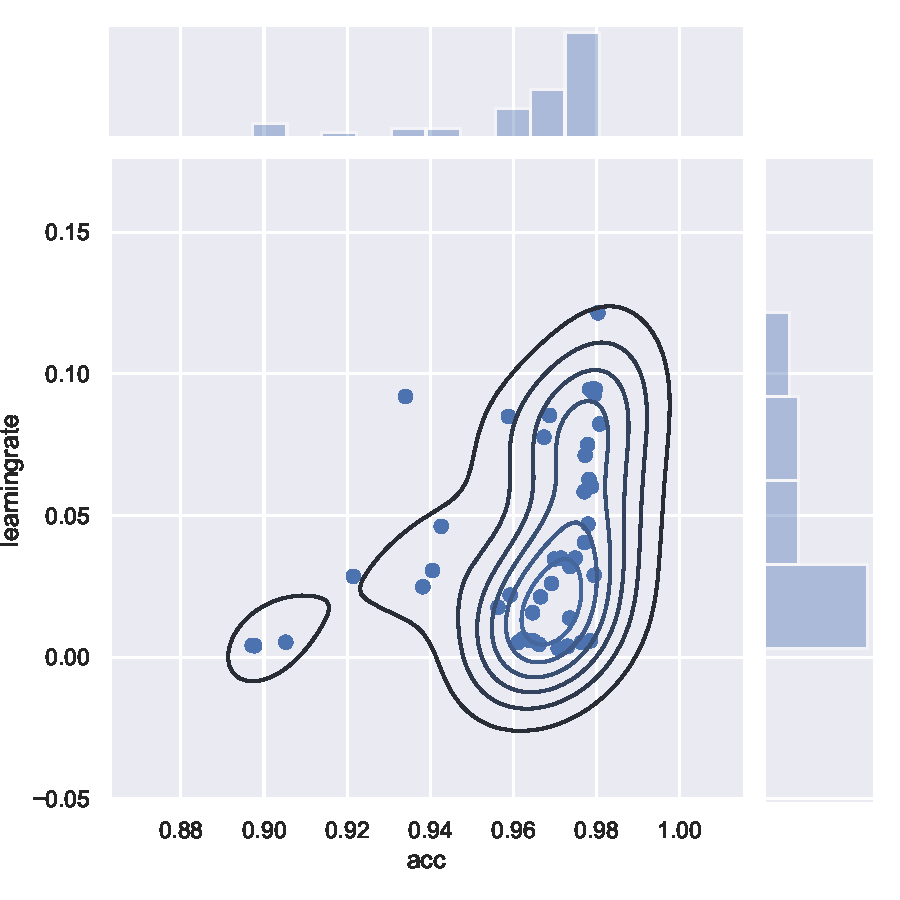
\includegraphics[scale=0.9]{img/hp_learningrate.pdf}
  \caption{Dichte-Diagramm der Lernrate in Verbindung mit der Klassifizierungsgenauigkeit(acc)}
  \label{fig:hp_learningrate}
\end{figure}

\subsection{Diagramm Dropout}
In Abbildung \ref{fig:hp_Dropout} ist der Dropout in Verbindung mit der Klassifizierungsgenauigkeit aufgetragen. Es zeigte sich ein Dropout im Bereich von 0,1 bis 0,4 als zielführend. Zudem ist der Dropout im Bereich von 0,2 in den Individuen der letzten Generation häufig vertreten, wodurch dies eine hohe Garantie für eine hochwertiges Individuum widerspiegelt. Im Diagramm ist auch gut zusehen, dass eine Dropoutrate über 0,5 sich kontraproduktiv für die Klassifzierungsgenauigkeit auswirkt. Dies ist über die geringe Klassifzierungsgenauigkeit(acc) für den Dropout über 0,5 sichtbar.

\begin{figure}[h]
  \centering  
  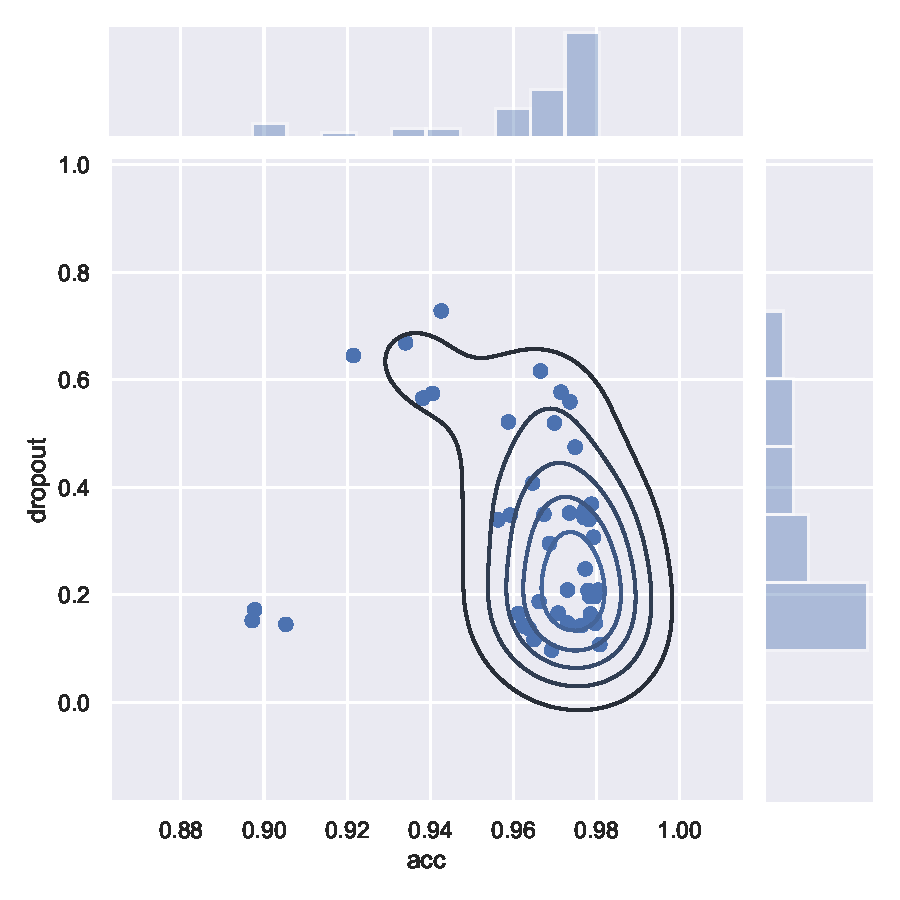
\includegraphics[scale=0.9]{img/hp_dropout.pdf}
  \caption{Dichte-Diagramm des Dropouts in Verbindung mit der Klassifizierungsgenauigkeit(acc)}
  \label{fig:hp_Dropout}
\end{figure}

\newpage

\subsection{Diagramm Batchsize}
In Abbildung \ref{fig:hp_Batchsize} ist die Batchsize in Verbindung mit der Klassifizierungsgenauigkeit aufgetragen. Es zeigte sich eine Batchsize im Bereich von 30 bis 50 als nützlich. Zudem ist die Batchsize im Bereich von 40 in den Individuen der letzten Generation häufig vertreten, wodurch dies eine hohe Garantie für ein hochwertiges Individuum widerspiegelt.

\begin{figure}[H]
  \centering  
  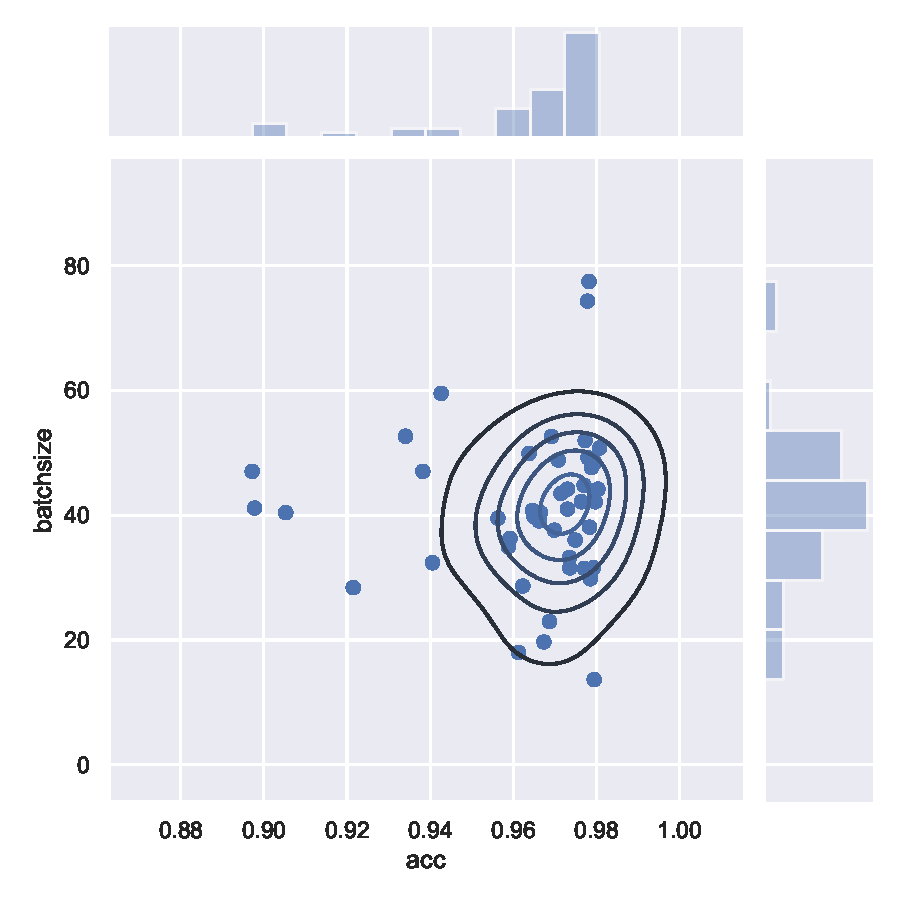
\includegraphics[scale=0.9]{img/hp_batchsize.pdf}
  \caption{Dichte-Diagramm der Batchsize in Verbindung mit der Klassifizierungsgenauigkeit(acc)}
  \label{fig:hp_Batchsize}
\end{figure}

\newpage

\subsection{Diagramm Epochen}
In Abbildung \ref{fig:hp_Epochen} ist die Epochenanzahl in Verbindung mit der Klassifizierungsgenauigkeit aufgetragen. Es zeigte sich, dass eine Epochenanzahl im Bereich von 20 bis 80 als zielführend. Zudem sind die Epochen im Bereich von 40 in den Individuen der letzten Generation häufig vertreten, wodurch dies eine hohe Garantie für eine hochwertiges Individuum widerspiegelt. In diesem Diagramm ist gut zusehen das ein Individuum mit höherer Epochenanzahl meist gute Fitnesswerte liefert, wobei eine geringere Epochenanzahl ab einem bestimmten Wert, hier 20, eine geringere Fitness aufweist.

\begin{figure}[H]
  \centering  
  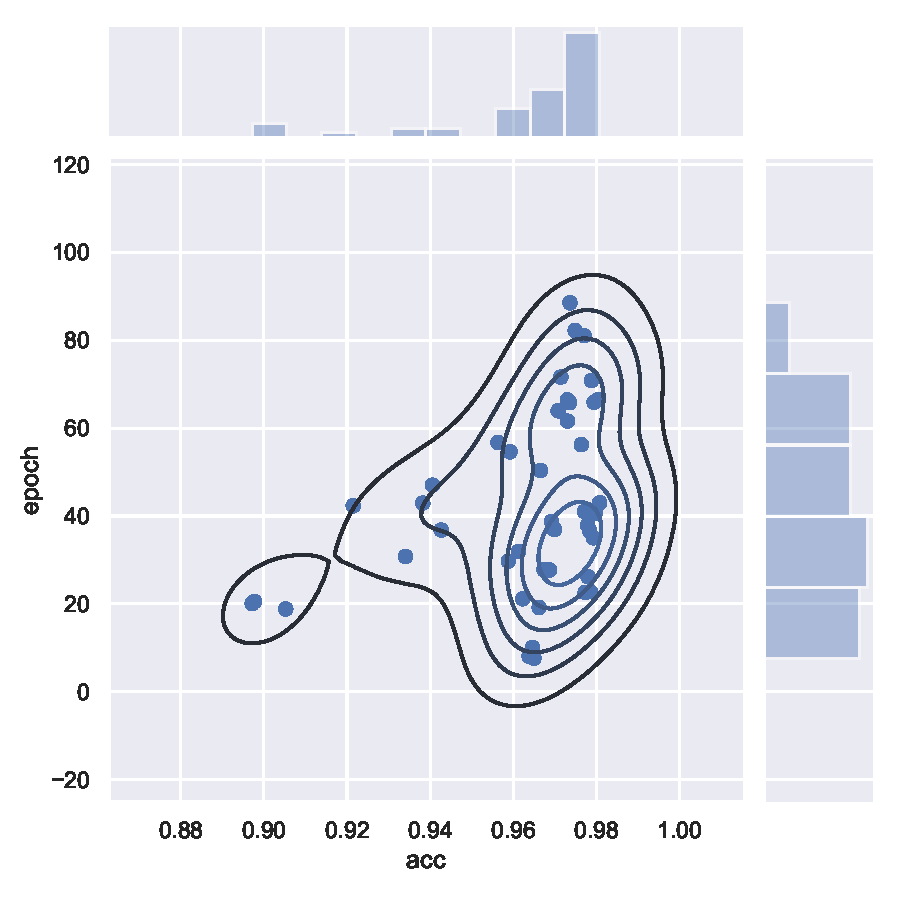
\includegraphics[scale=0.9]{img/hp_epoch.pdf}
  \caption{Dichte-Diagramm die Epochenanzahl in Verbindung mit der Klassifizierungsgenauigkeit(acc)}
  \label{fig:hp_Epochen}
\end{figure}

\newpage

\subsection{Diagramm Optimierer}
In Abbildung \ref{fig:hp_Optimierer} sind die Optimierer in Verbindung mit der Klassifizierungsgenauigkeit aufgetragen. Es zeigte sich, dass der Optimierer 1 = SGD und 3 = Adagrad am häufigsten mit gutem Fintesswert auftreten. Es ist gut zusehen, das einzelne Optimierer wie 2 = RMSporp oder 7 = ftrl gar nicht auftreten, dementsprechend schneiden diese Optimierer schlecht ab. Somit erhalten wir durch das Dichte-Diagramm, dass SGD und Adagrad die favorisierten Optimierer sind.

\begin{figure}[H]
  \centering  
  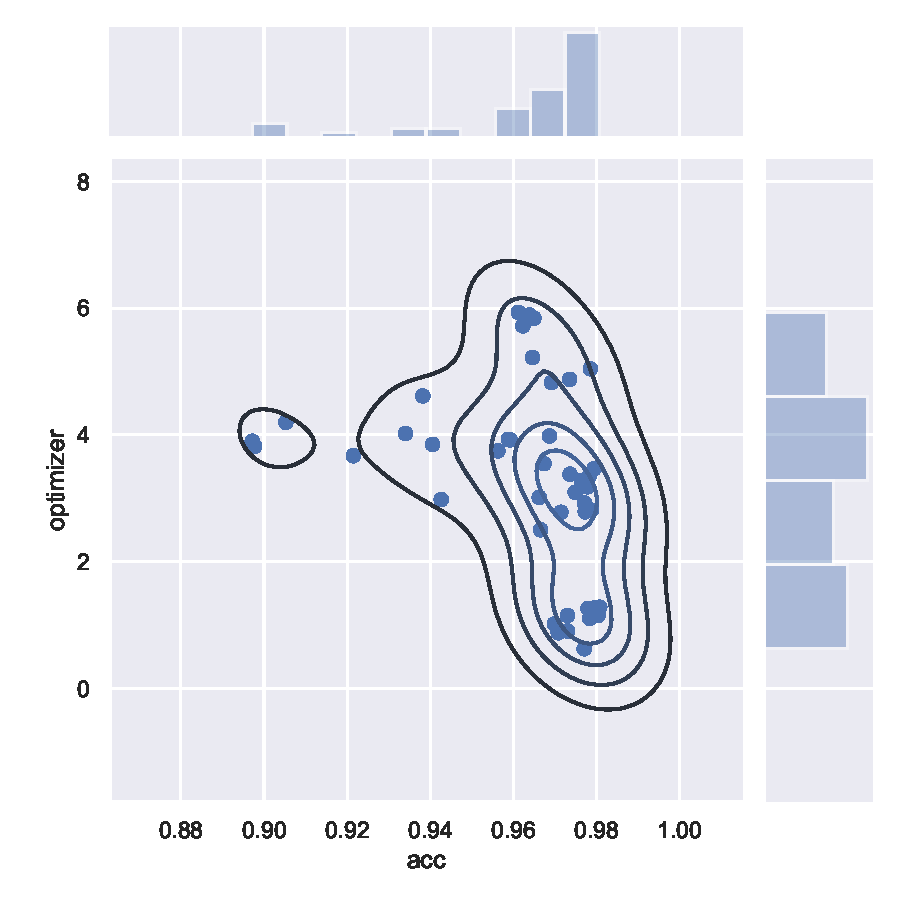
\includegraphics[scale=0.9]{img/hp_optimizer.pdf}
  \caption{Dichte-Diagramm der Optimierer in Verbindung mit der Klassifizierungsgenauigkeit(acc)}
  \label{fig:hp_Optimierer}
\end{figure}
Jede ganze Zahl des Optimizer steht für einen eigenen Optimierer. Es gilt: 0=adam, 1=SGD, 2=RMSprop, 3=Adagrad, 4=adadelta, 5=adammax, 6=nadam, 7=ftrl.

\newpage

\section{Diskussion der Ergebnisse}
Bei den Optimierungen der Hyperparameter haben sich nicht die erwarteten Ergebnisse gezeigt. Bei der Optimierung der Hyperparameter der Fully Connected Netze zeigten sich nur sehr geringe Unterschiede in den Ergebnissen. Diese Unterschiede liegen im Nachkommabereich und können vernachlässigt werden. Somit konnte bei der Optimierung des Fully Connected keiner der Algorithmen sich als besser herausstellen. Bei der Hyperparameter Optimierung ergaben sich ähnliche Ergebnisse. Bei 250 Iterationen war die Zufallssuche sogar bis zu 4\% besser als der GA. Bei der Hyperparameteroptimierung mit kleinem Datensatz waren eine Verbesserung von bis zu 1\% beim Fully Conntected Netz mit Hilfe des GA möglich, dennoch ist diese Verbesserung irrelevant klein. Somit konnten in allen drei Optimierungsversuchen keine relevante Verbesserung der Klassifikationsgenauigkeit mit Hilfe des Genetischen Algorithmus gegenüber der Zufallssuche gezeigt werden. Dabei äußerte sich eine Änderung der Berechnungsdauer sowie der Modell-Architektur nicht in einer Änderung der Endergebnisse. Die geringe Verbesserung liegt nicht daran, dass der GA ungeeignet ist. Denn der GA konnte im Vergleich zur Zufallssuche häufiger Individuen finden, welche einen guten Fitnesswert besitzen. Dennoch gab es kein Individuum das verbesserte Ergebnisse lieferte. Somit konnte die Zufallssuche mit ihren wenigen gefundenen Individuen die gleiche Ergebnisse erreichen wie der GA. Dies kann durch einen geringen Einfluss der Hyperparameter auf das Endergebnis begründet werden. Kleine Veränderungen der Hyperparameter haben keine messbaren Änderungen der Endergebnisse ergeben. Solange die Hyperparameter in einem bestimmten Rahmen liegen, werden gute Klassifizierungsergebnisse erzielt. Dieser Rahmen für die Hyperparameter kann mit Hilfe des GA sichtbar gemacht werden. Durch die Population im GA kann gesagt werden in welchem Rahmen sich die Hyperparameter befinden müssen um gute Ergebnisse zu liefern. Diese Information konnte aus der Zufallssuche nicht entnommen werden, da die meisten Individuen der Zufallssuche keinen guten Fitnesswert besitzen. Dieser Rahmen zeigt sich in der Auswertung über die Visualisierung \ref{ssec:Visualisierung}, somit erreicht der Genetische Algorithmus gegenüber der Zufallssuche keine großen Verbesserungen. Doch durch seine Zusatzinformationen kann ein Mehrwert mit gleicher Berechnungszeit gewonnen werden.

\newpage

\section{Zusammenfassung}
In diesem Kapitel wurde auf die Ergebnisse und deren Auswertung eingegangen. Dazu wurden zuerst die Benchmarks des Trainingsvorgangs erklärt. Es zeigte sich, dass große KNNs deutlich schneller auf der GPU trainieren. Hingegen trainieren kleine KNNs auf der CPU deutlich schneller. Anschließend werden die Ergebnisse des Evaluierungsteils besprochen. Hier zeigten sich nicht die erwarteten Ergebnisse. Der Genetische Algorithmus konnte nur in wenigen Fällen eine Verbesserung der Klassifkationsergebnisse, über das Optimieren der Hyperparameter, erreichen. Zudem war die Verbesserungen vernachlässigbar klein. Denn die Zufallssuche konnte wenige Individuen mit guten Hyperparametern finden. Diese Individuen waren ausreichend gut, dass eine Optimierung mit Hilfe des GA keine Verbesserung gegenüber diesen Individuen erbrachte. Dennoch hat der Genetische Algorithmus einen Vorteil. Er kann über seine letzte Population eine zusätzliche Aussage treffen. Diese beinhaltet in welchen Bereichen sich die einzelnen Hyperparameter befinden, die gute Ergebnisse liefern. Diese Bereiche wurden mithilfe des Dichte-Diagramms sichtbar gemacht.